\documentclass{article}[11pt,a4paper]

\usepackage[utf8]{inputenc}
\usepackage[T1]{fontenc}
\usepackage[frenchb]{babel}


\usepackage{hyperref}
\usepackage{graphicx} %pour integrer des images
\usepackage{layout} %pour avoir les informations de mise en page
\usepackage{soul} %soulignement et texte barrer
\usepackage{ulem} %soulignement
\usepackage{amsmath}
\usepackage{amssymb}
\usepackage{mathrsfs}
\usepackage{moreverb} %idem
\usepackage{listings} %citation de code colore (ne pas oublier de le parametrer correctement \lstset
\usepackage{color} %couleur du texte a utiliser avec prudence et retenue
\usepackage{eurosym} %permet l'utilisation du symbole euro
\usepackage{numprint}
\usepackage{fancyhdr}
\usepackage[table]{xcolor}
\usepackage{graphicx}
%\usepackage{subscript}
\makeatletter
\newcommand{\nbSecondes}{2 (à définir)}%temps pour les infections
\newcommand{\porteeParDefaut}{1}%portée des bombes au début de la partie

% Définition de couleurs personnalisées
\definecolor{blueTab}{RGB}{138,245,255}


\def\clap#1{\hbox to 0pt{\hss #1\hss}}%
\def\ligne#1{%
\hbox to \hsize{%
\vbox{\centering #1}}}%
\def\haut#1#2#3{%
\hbox to \hsize{%
\rlap{\vtop{\raggedright #1}}%
\hss
\clap{\vtop{\centering #2}}%
\hss
\llap{\vtop{\raggedleft #3}}}}%
\def\bas#1#2#3{%
\hbox to \hsize{%
\rlap{\vbox{\raggedright #1}}%
\hss
\clap{\vbox{\centering #2}}%
\hss
\llap{\vbox{\raggedleft #3}}}}%
\def\maketitle{%
\thispagestyle{empty}\vbox to \vsize{%
\haut{}{\@blurb}{}
\vfill
\vspace{1cm}
\begin{flushleft}
\usefont{OT1}{ptm}{m}{n}
\huge \@title
\end{flushleft}
\par
\hrule height 4pt
\par
\begin{flushright}
\usefont{OT1}{phv}{m}{n}
\large \@author
\par
\end{flushright}
\vfill
\begin{center}

\includegraphics[scale=0.5]{images/logo.png}
\end{center}
\vfill
\bas{Info 3}{\@date}{\@location}
}%
\cleardoublepage
}
\def\date#1{\def\@date{#1}}
\def\author#1{\def\@author{#1}}
\def\title#1{\def\@title{#1}}
\def\location#1{\def\@location{#1}}
\def\blurb#1{\def\@blurb{#1}}
\date{Année 2011 - 2012}
\author{}
\title{}
\location{Nantes}\blurb{}
\makeatother
\title{Projet Bomberman - \textit{Cahier des charges}}
\author{\textbf{Bisiaux} Alexandre\\\textbf{Guihal} Maxime\\\textbf{Guillermic} Brice\\\textbf{Rousseau} Simon}
\location{Nantes}
\blurb{%
École polytechnique de l'Université de Nantes\\
Département informatique
}% 
\setlength{\textwidth}{385pt}
\setlength{\oddsidemargin}{42pt}
\pagestyle{fancy}
\fancyhead{}
\rhead{\textsc{Projet Bomberman}}
\lhead{\textsc{Bisiaux - Guihal - Guillermic - Rousseau}}



\begin{document}
%\renewcommand{\sectionname}{Partie} % changer "chapitre" pour "partie"
%\layout
\maketitle

\tableofcontents
\newpage

\section*{Présentation du projet}\addcontentsline{toc}{section}{Présentation du projet}
Ce document présente la conception choisie pour le programme. Celui-ci est découpé en 5 modules distincts pouvant être développés séparément. Chacun de ces modules est décrit ci-après, et est accompagné de diagrammes UML permettant de représenter sa structure interne, et externe, ainsi que son mode de fonctionnement.

\vspace{0.5cm}

\subsection{Bibliothèques utilisées}

Ce programme sera réalisé à l'aide du langage \textbf{C++}. La bibliothèque graphique utilisée sera la \textbf{SFML 1.6} choisie pour sa simplicité et son efficacité. Celle-ci est sous licence zlib/png qui permet son utilisation sans aucune contreparties.

\newpage

\section{Règles du jeu}
\subsection{But du jeu}

Le but principal du jeu Bomberman est d'être le dernier survivant de la partie. Des joueurs sont répartis sur une carte et doivent déposer des bombes de façon stratégique afin d'éliminer les autres joueurs en les faisant exploser.

Le jeu se joue sous forme de match composé d'un nombre inconnu de parties. A la fin de chaque partie, l'ordinateur ayant créé la partie choisit de continuer ou de recommencer un match. Chaque partie rapporte un point à son vainqueur (le dernier à rester en vie). Le match est gagné par le joueur qui a accumulé le plus de points au cours des parties.

\subsection{Nombre de joueurs}

Le nombre de joueurs doit être d'un minimum de 2 et d'un maximum de 4. Ces joueurs peuvent jouer sur un ou plusieurs ordinateurs en réseau.

\subsection{Déroulement d'une partie}

\subsubsection{Situation initiale}

La carte est une carte rectangulaire de 19 cases horizontales et 13 cases verticales. Chaque case est remplie par une entité de jeu contenue dans cette liste (lors d'un début de partie, les cases ne peuvent être remplie que par les 4 premières entités) :

\begin{itemize}
    \item Vide
    \item Personnage
    \item Mur indestructible
    \item Caisse à exploser
    \item Bombe
    \item Bonus
    \item Déflagration de bombe
\end{itemize}

Les joueurs sont placés selon le nombre de joueurs : 
\begin{itemize}
\item \textbf{4 joueurs} : Les joueurs sont placés dans les 4 coins de la carte.
\item \textbf{3 joueurs} : 2 joueurs sont placés dans les coins supérieurs et le troisième est placé sur la dernière ligne au centre.
\item \textbf{2 joueurs} : Un joueur se trouve dans le coin supérieur gauche, le deuxième dans le coin inférieur droit.
\end{itemize}

Au début, chaque joueur sera dans une zone avec au moins 3 cases vides consécutives afin de pouvoir faire exploser au moins une bombe. De plus, les joueurs ne peuvent poser qu'une bombe à la fois, se déplacent à vitesse normale et les bombes ont une portée de \porteeParDefaut .

\subsubsection{Déroulement}

Les joueurs ainsi que des caisses sont réparties sur la carte selon le nombre de joueurs et les paramètres. Ensuite, la partie démarre. Les joueurs peuvent poser des bombes afin de détruire des caisses. À chaque destruction de caisse, il peut y avoir un bonus qui apparaît. Si la déflagration d'une bombe touche un joueur (que se soit son poseur ou un autre joueur), ce joueur est considéré comme mort et disparaît de la carte. Tant qu'il reste des caisses, la portée des bombes dépend des bonus pris par le bomberman. Une fois toutes les caisses détruites, la portée des bombes devient maximale et les déflagrations traversent toute la carte.

\subsubsection{Fin de partie}

La partie est terminée lorsqu'il n'y a plus qu'un survivant sur la carte. Dans le cas où il n'y aurait pas de survivant (les derniers joueurs meurent à la suite de l'explosion des dernières bombes), la partie est considérée comme nulle.

\subsection{Bonus - Malus}

Il existe différents types de bonus. Certains améliorent ou bien dégradent les caractéristiques des bombes des joueurs, d'autres celles des personnages. Il existe aussi des "infections" qui sont des malus qui affectent un ou plusieurs joueurs.

\subsubsection{Bonus pour les bombes}

Les bonus et malus disponibles pour les bombes seront :
\begin{itemize}
\item \textbf{Bombe Up} : Augmentation du nombre de bombes pouvant être posées simultanément par un joueur
\item \textbf{Bombe Down} : Diminution du nombre de bombes pouvant être posées simultanément par un joueur
\item \textbf{Flamme Jaune} : Augmentation de la portée d'une bombe d'une case
\item \textbf{Flamme Bleue} : Diminution de la portée d'une bombe d'une case
\item \textbf{Flamme Rouge} : Augmentation de la portée de la bombe au maximum
\item \textbf{Mine} : Bombe qui se déclenche lorsqu'un joueur marche dessus
\item \textbf{Bombe à pics} : Bombe dont la déflagration ne s'arrêtent pas lorsqu'elle rencontre une caisse
\item \textbf{Bombe atomique} : Explosion circulaire qui explose en 8-connexité d'une portée celle du joueur
\end{itemize}

Quand un joueur obtient le bonus \emph{Mine}, il peut n'en poser qu'une seule sur la carte avant que le bonus soit annulé.

\subsubsection{Bonus pour les personnages}

Les bonus et malus disponibles pour les personnages seront :
\begin{itemize}
\item \textbf{Patins} : Augmentation de la vitesse de déplacement du personnage
\item \textbf{Sabots} : Diminution de la vitesse de déplacement du personnage
\item \textbf{Ligne de bombes} : Une option qui permet au personnage de poser toutes ses bombes d'un seul coup, alignées devant lui,
\item \textbf{Détonateur} : Ce bonus permet de transformer toutes les bombes posées en bombes télécommandées. - 1 fois, juste nos bombes
\end{itemize}

\subsubsection{Infections}

Les infections disponibles seront :
\begin{itemize}
\item \textbf{Crâne} : Infection aléatoire parmi les infections ci-dessous
\item \textbf{Enfer} : Tous les personnages sont touchés par une infection aléatoire
\item \textbf{Confusion} : Inversion des touches du clavier
\item \textbf{Spasmes} : Mouvement vers une case tous les \nbSecondes secondes
\item \textbf{Dilatation} : Lenteur du personnage au maximum
\item \textbf{Fureur} : Pose une bombe toutes les \nbSecondes secondes
\end{itemize}

Une infection prend fin quand le personnage attrape un autre bonus.

\subsubsection{Probabilités des bonus - malus}

\begin{figure}[h]
	\begin{center}
		\begin{tabular}{|r|c|}
		\hline 
		& Probabilités \\ 
		\hline 
		Bonus pour les bombes & \% \\ 
		\hline 
		Bonus pour le personnage & \% \\ 
		\hline 
		Infections & \% \\ 
		\hline 
		\end{tabular} 
	\end{center}
	\caption{Probabilité des catégories}
\end{figure}

\begin{figure}[h]
	\begin{center}
		\begin{tabular}{|r|c|}
\hline 
& Probabilités \\ 
\hline 
Bombe Up & • \\ 
\hline 
Bombe Down & • \\ 
\hline 
Flamme Jaune & • \\ 
\hline 
Flamme Bleue & • \\ 
\hline 
Flamme Rouge & • \\ 
\hline 
Mine & • \\ 
\hline 
Bombe à pics & • \\ 
\hline 
Bombe atomique & • \\ 
\hline 
\end{tabular} 
	\end{center}
	\caption{Probabilité des bonus pour les bombes}
\end{figure}

\begin{figure}[h]
	\begin{center}
		\begin{tabular}{|r|c|}
\hline 
& Probabilités \\ 
\hline 
Patins & • \\ 
\hline 
Sabots & • \\ 
\hline 
Ligne de bombes & • \\ 
\hline 
Détonateur & • \\ 
\hline 
\end{tabular} 
	\end{center}
	\caption{Probabilité des bonus pour les personnages}
\end{figure}

\begin{figure}[h]
	\begin{center}
		\begin{tabular}{|r|c|}
\hline 
& Probabilités \\ 
\hline 
Crâne & • \\ 
\hline 
Devil & • \\ 
\hline 
Confusion & • \\ 
\hline 
Spasmes & • \\ 
\hline 
Dilatation & • \\ 
\hline 
Fureur & • \\ 
\hline 
\end{tabular} 
	\end{center}
	\caption{Probabilité des infections}
\end{figure}

\newpage

\section{Interface graphique}
\subsection{Présentation de l'interface graphique}

Lorsque le programme démarrera, une fenêtre d'une taille de 800 pixels de largeur sur 600 pixels de hauteur apparaîtra représentant pendant quelques secondes l'écran d'accueil du programme, c'est-à-dire une image occupant tout la fenêtre nommant le programme et présentant éventuellement les noms des créateurs. Un fondu laissera ensuite apparaître le menu principal.

\subsection{Menus}

Pour chaque menu présenté ci-dessous, les options affichées seront sélectionnables grâce aux touches directionnelles haut et bas du clavier. L'option  actuellement sélectionnée sera représentée d'une manière différente, en changeant sa couleur, ou en affichant un curseur devant elle. La validation de l'option sélectionnée s'effectuera par pression de la touche \emph{Entrée}. Un appui sur la touche \emph{Echap} permettra de revenir sur l'ecran de menu précédent.

\subsubsection{Menu principal}

Le menu principal présentera trois options à l'utilisateur : \emph{Jouer}, \emph{Options}, \emph{Quitter}, permettant respectivement d'aller sur le menu de jeu, de paramétrage, ou de quitter le programme sans confirmation. Le nom du jeu sera également visible au-dessus de ces options. Sur ce menu, la touche \emph{Echap} n'aura pas d'effet.

\subsubsection{Menu de paramétrage}

Ce menu permettra à l'utilisateur de pouvoir régler les options générales du programme. Il présentera une option \emph{Contrôles} permettant de configurer les contrôleurs et les touches de jeu, comme défini dans le prochain paragraphe. Il affichera en plus une option \emph{Audio} permettant d'aller sur le menu de configuration audio. Enfin, la dernière option \emph{Graphisme} permettra de changer les options graphiques du jeu en allant sur le menu du même nom. Une option \emph{Retour} pour retourner au menu principal sera également affichée.

\paragraph{Menu de configuration des contrôleurs}

Ce menu permettra de gérer l'attribution des touches pour chaque joueur. Un premier ecran listera les quatre joueurs en précisant le type de contrôleur utilisé. Une option \emph{Retour} pour retourner au menu de paramétrage sera également affichée. Lorsque l'utilisateur sélectionnera un joueur, un second ecran s'affichera. Celui-ci présentera en haut de la fenêtre un widget de sélection d'un contrôleur (clavier, joystick ou Wiimote) où le nom du contrôleur est affichée entourée de deux flèches permettant de sélectionner le contrôleur précédent ou suivant de l'actuel avec les flèches directionnelles gauche et droite. En dessous de ce widget se trouvera soit une image représentant le contrôleur avec l'emplacement des boutons prédéfinis pour la Wiimote, soit une liste des actions possibles avec l'assignation de la touche à côté. Lorsque l'action sera sélectionnée puis validée, le programme attendra que l'utilisateur saisisse la touche pour l'assigner. Lorsque l'utilisateur voudra assigner une touche déjà assignée, le programme affichera un message d'erreur informant l'utilisateur que la touche est déjà assignée. Sur cet ecran, un bouton de retour vers le menu qui liste les joueurs.

\paragraph{Menu de configuration audio}

Ce menu gérera le volume de la musique et des effets sonores du jeu et du menu avec deux widgets permettant à l'utilisateur de choisir le volume entre 0\% et 100\%. Un bouton permettant de couper directement le son sera présent à côté de chacun des widgets. Un bouton de retour au menu précédent sera également visible.

\paragraph{Menu de configuration graphique}

Ce menu permettra de configurer l'aspect graphique du jeu. Il présentera une option permettant de passer du mode fenêtré au mode plein écran. En-dessous se trouvera un widget permettant de choisir le pack de textures à utiliser pour le programme. Celui-ci listera les packs disponibles et l'utilisateur pourra en sélectionner un. Un bouton permettant de revenir au menu de paramétrage sera aussi présent.

\subsection{Plateau de jeu}



\newpage

\section{Gestion des contrôleurs de jeu}
Chaque joueur peut choisir son contrôleur de jeu via les options du menu. Il a le choix entre ces différents périphériques :

\begin{itemize}
	\item le clavier
	\item Joystick
	\item wiimote
\end{itemize}
	
	
\subsubsection{Clavier}
Il est possible de paramétrer les différentes commandes du jeu en passant par le menu.

Par défaut les commandes du jeu sont les suivantes :

\begin{center}
	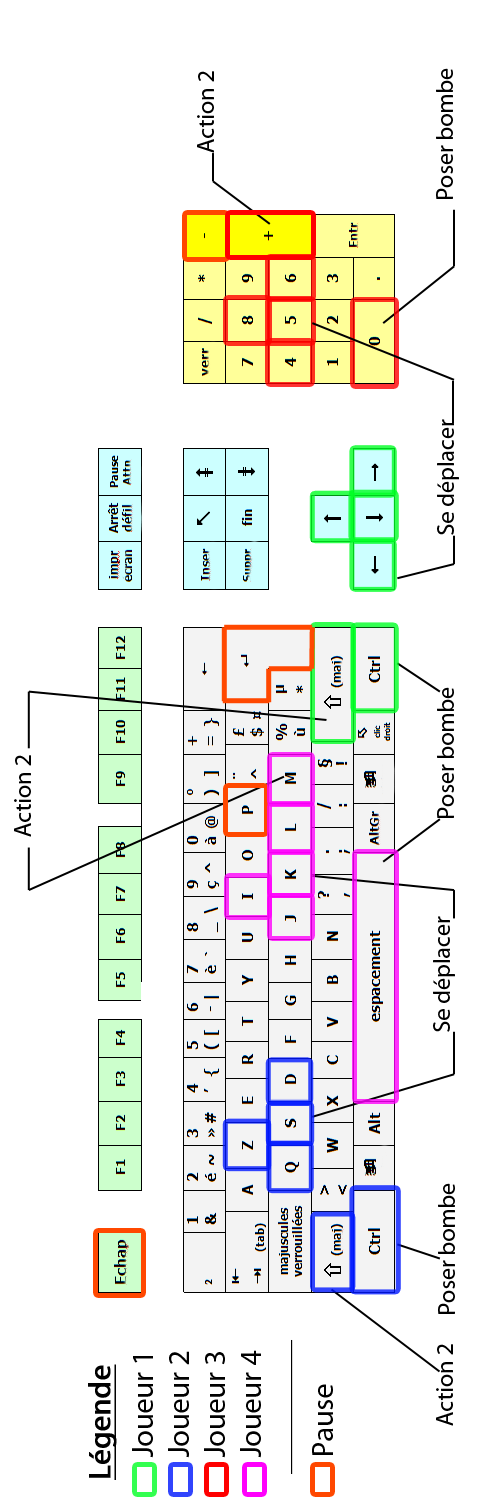
\includegraphics[height=550pt]{images/clavier}
\end{center}

\subsubsection{Joystick}
La prise en charge des contrôleurs de jeu PC de type Joystick se fait par l'intermédiaire de la librairie SFML.

Comme le clavier, il est possible de paramétrer les différentes commandes du jeu en passant par le menu.

Par défaut les commandes du jeu sont les suivantes :

\begin{center}
	\begin{tabular}{|c|c|}
		\hline
			\rowcolor{blueTab}
			\textbf{Action} & \textbf{Touche(s)} \\
		\hline
		Se déplacer & Pad directionnel \\
		\hline
		Poser une bombe & Bouton 1\\
		\hline
		Action 2 & Bouton 2\\
		\hline
	\end{tabular}
\end{center}


\subsubsection{Wiimote}
La prise en charge d'un contrôleur de type Wiimote se fait par l'intermédiaire de la librairie Wiiusecpp. Cette librairie sous licence GNU GPLv3 et GNU LGPLv3 (non commercial) est codée en langage C++ et est principalement basée sur la librairie Wiiuse. La librairie est disponible pour les systèmes d'exploitation Linux et Windows.

Le jeu ne requiert pas l'utilisation du nunchuck.

Les commandes de jeu sont les suivantes et ne peuvent être modifiées :

\begin{center}
	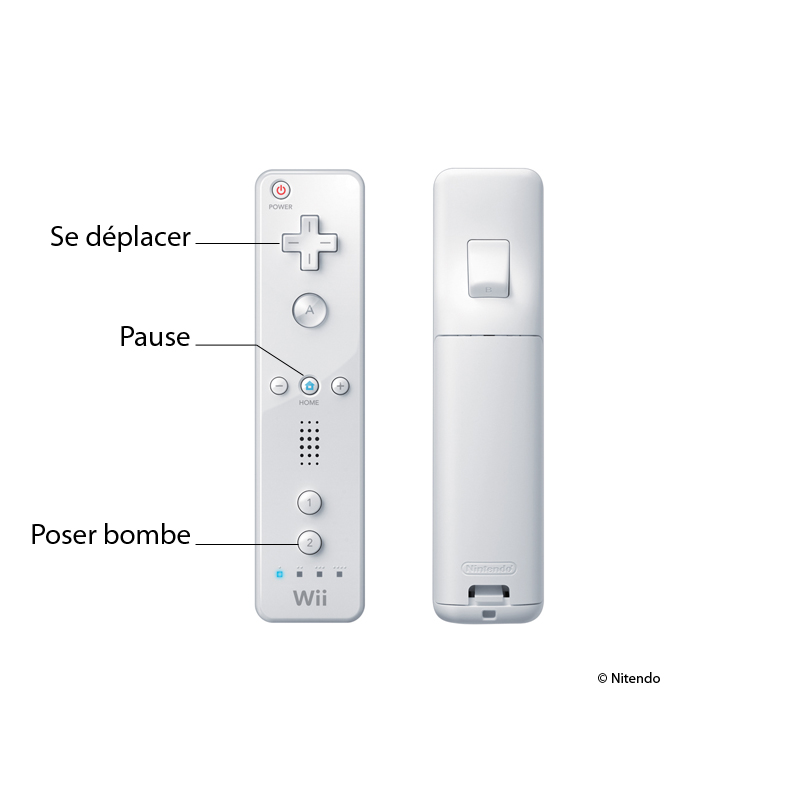
\includegraphics[scale=1.7]{images/wiimote}
\end{center}

\newpage

\section{Gestion du réseau}
Le jeu du bomberman doit permettre aux différents joueurs de se connecter en réseau afin de pouvoir participer à la même partie par l'intermédiaire d'un autre ordinateur. Il faut donc mettre en place un réseau qui donne la possibilité de jouer en réseau. 

\subsection{Système centralisé}
C'est le système centralisé qui a été retenu pour ce jeu, contrairement au réseau décentralisé. L'avantage de ce système est qu'un ordinateur central fera office de serveur et distribuera la même information aux autres postes connectés. Toutes les informations doivent donc être rapatriées vers ce serveur qui calculera les données et les renverra à tous les postes. De cette façon, on peut avoir la certitude qu'à un moment donné, tous les ordinateurs ont la même information.

\subsection{Synchronisation de l'information}
Un des problèmes des réseaux est le temps d'acheminement de l'information d'un poste à un autre. Ce temps diffère en fonction du trafic mais aussi en fonction de la distance à parcourir. Cela peut provoquer, à l'arrivée, un décalage entre les différents postes de jeu. Afin d'y remédier, le jeu devra être synchronisé pour que chaque modification transmise sur le réseau soit prise en compte en même temps et ainsi favoriser la jouabilité en réseau.

\subsection{Informations transmises}
Lors d'une partie, l'ordinateur ayant le rôle de serveur s'occupera de gérer le jeu en lui-même. Les informations communiquants sur le réseau seront donc de deux types. D'une part les informations fournies par les ordinateurs clients concernant les touches saisies pour chaque contrôleur de jeu, seront envoyées vers le serveur. D'autre part, le serveur, après avoir géré la partie en fonctions des informations reçues, envoie à chaque ordinateur client les informations d'affichage de la partie.


\newpage

\section*{Conclusion}\addcontentsline{toc}{section}{Conclusion}
Cette description de chaque module est suivie en annexe des diagrammes de classes correspondants, ainsi que du diagramme de composants et de déploiement du programme.\\

Cette conception est susceptible d'évoluer au cours du développement du programme. Elle donne juste une vue globale de la structure du projet.\\

Pour les diagrammes de classes, la légende des couleurs est la suivante :

\begin{itemize}
    \item \textbf{Bleu} : Classe
    \item \textbf{Vert} : Interface fournie
    \item \textbf{Orange} : Interface requise
    \item \textbf{Jaune} : Structure
    \item \textbf{Violet} : Enumération
    \item \textbf{Gris} : Classe déjà implémentée
\end{itemize}


\end{document}
